\documentclass[aspectratio=169]{beamer}
\input{shared/preamble}
\title{
    Electricidad I:\\
    \alert{\emph{Estructura atómica,}}\\
    \alert{\emph{carga eléctrica y}}\\
    \alert{\emph{campo eléctrico}}
}
\begin{document}
\input{shared/postamble}

\begin{frame}{Estructura atómica}
    \begin{columns}[onlytextwidth]
    \begin{column}{0.6\textwidth}
        \alert{\elementname{H}}\\[8pt]
        Número atómico: \atomicnumber{H}\\[8pt]
        Configuración electrónica:\\[8pt] 
        \elconf{H}\\[8pt]  
        \end{column}
    \begin{column}{0.4\textwidth}
    \begin{center}
        Modelo de Bohr:\\[8pt]
        \bohr{}{H}
    \end{center}
\end{column}
\end{columns}
\end{frame}

\begin{frame}{Estructura atómica}
    \begin{columns}[onlytextwidth]
    \begin{column}{0.6\textwidth}
        \alert{\elementname{Cu}}\\[8pt]
        Número atómico: \atomicnumber{Cu}\\[8pt]
        Configuración electrónica:\\[8pt] 
        \elconf{Cu}\\[8pt]  
        \end{column}
    \begin{column}{0.4\textwidth}
    \begin{center}
        Modelo de Bohr:\\[8pt]
        \bohr{}{Cu}
    \end{center}
\end{column}
\end{columns}
\end{frame}

\begin{frame}{Estructura atómica}
    \begin{columns}[onlytextwidth]
    \begin{column}{0.6\textwidth}
        \alert{\elementname{Si}}\\[8pt]
        Número atómico: \atomicnumber{Si}\\[8pt]
        Configuración electrónica:\\[8pt] 
        \elconf{Si}\\[8pt]  
        \end{column}
    \begin{column}{0.4\textwidth}
    \begin{center}
        Modelo de Bohr:\\[8pt]
        \bohr{}{Si}
    \end{center}
\end{column}
\end{columns}
\end{frame}

\begin{frame}{Materiales aislantes, semiconductores y conductores}
    \begin{center}
        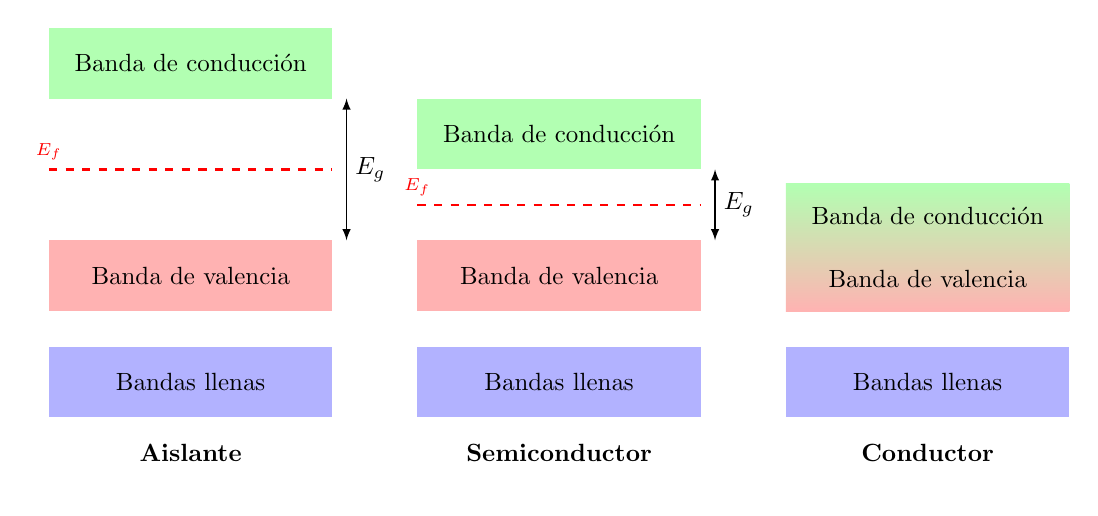
\begin{tikzpicture}[scale=0.9, transform shape]
            \begin{scope}
                \fill[green!30] (0,3) rectangle +(4,1) node[black,midway]{Banda de conducción}; 
                \fill[red!30] (0,0) rectangle +(4,1) node[black,midway]{Banda de valencia}; 
                \draw[dashed,thick,red] (0,2)node[above]{\scriptsize$E_f$} --++ (4,0);
                \draw[latex-latex] (4.2,1) --++ (0,2) node[midway,right]{$E_g$};
                \fill[blue!30] (0,-1.5) rectangle +(4,1) node[black,midway]{Bandas llenas};
                \fill[white] (0,-2.5) rectangle +(4,1) node[black,midway]{\textbf{Aislante}};
            \end{scope}
            \begin{scope}[xshift=5.2cm]
                \fill[green!30] (0,2) rectangle +(4,1) node[black,midway]{Banda de conducción}; 
                \fill[red!30] (0,0) rectangle +(4,1) node[black,midway]{Banda de valencia};
                \draw[dashed,thick,red] (0,1.5)node[above]{\scriptsize$E_f$} --++ (4,0);
                \draw[latex-latex] (4.2,1) --++ (0,1) node[midway,right]{$E_g$};
                \fill[blue!30] (0,-1.5) rectangle +(4,1) node[black,midway]{Bandas llenas};
                \fill[white] (0,-2.5) rectangle +(4,1) node[black,midway]{\textbf{Semiconductor}};
            \end{scope}
            \begin{scope}[xshift=10.4cm]
                \shade[top color=green!30,bottom color=red!30] (0,0) rectangle +(4,1.8);
                \draw (2,1.35) node[black]{Banda de conducción};
                \draw (2,0.45) node[black]{Banda de valencia};
                %\fill[red!30] (0,0) rectangle +(4,1) node[black,midway]{Banda de valencia};
                \fill[blue!30] (0,-1.5) rectangle +(4,1) node[black,midway]{Bandas llenas};
                \fill[white] (0,-2.5) rectangle +(4,1) node[black,midway]{\textbf{Conductor}};
            \end{scope}
        \end{tikzpicture}
    \end{center}
\end{frame}

\begin{frame}{Carga eléctrica} 
    \begin{columns}[onlytextwidth]
    \begin{column}{0.6\textwidth}
        La carga eléctrica es una propiedad de las particulas atómicas de las que se compone la materia, se mide en coulombs (\si{\coulomb})\\[4pt]
        La carga del electrón equivale a \SI{-1.602e-19}{C}
    \end{column}
    \begin{column}{0.4\textwidth}
        \begin{center}
            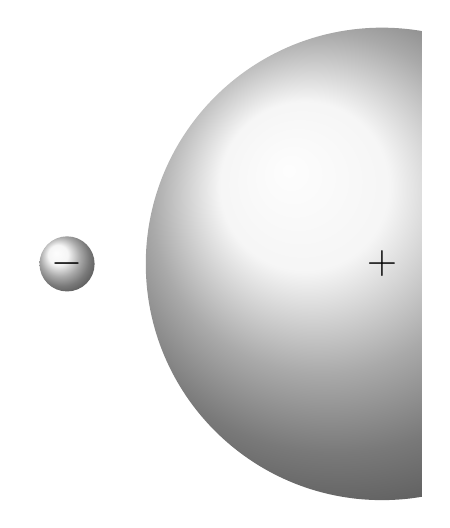
\begin{tikzpicture}[scale=1]
                \clip (-2.5,-3) rectangle (2.5,3);
                \coordinate (e) at (-2,0);
                \coordinate (p) at (2,0);
                \shade[ball color=gray!10!] (e) circle (.35) node{\Large$-$};
                \shade[ball color=gray!10!] (p) circle (3) node{\Large$+$};
            \end{tikzpicture}
        \end{center}
    \end{column}
    \end{columns}
\end{frame}

\begin{frame}{Fuerza eléctrica} 
    \begin{columns}[onlytextwidth]
    \begin{column}{0.6\textwidth}
        La fuerza eléctrica es la fuerza de atracción o repulsión entre dos cuerpos o partículas cargadas 
        \begin{equation*}
            F = k\dfrac{q_1q_2}{r^2}
        \end{equation*}
        donde $F$ es la fuerza eléctrica en newtons (\si{\newton}), $k$ es la constante de Coulomb ($\SI{9e9}{\newton \meter\squared / \coulomb \squared}$), $q_1$ y $q_2$ son dos cargas en coulombs (\si{\coulomb}), y $r$ es la distancia que separa a las cargas en metros (\si{\meter})   
    \end{column}
    \begin{column}{0.4\textwidth}
        \begin{center}
            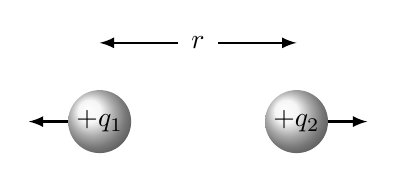
\begin{tikzpicture}[scale=1]
                \shade[ball color=gray!10!] (0,0) coordinate(q1) circle (.4) node{$+q_1$};
                \shade[ball color=gray!10!] (2.5,0) coordinate(q2) circle (.4) node{$+q_2$};
                \draw[-latex,thick] (q1)++(-0.4,0)--+(-0.5,0);
                \draw[-latex,thick] (q2)++(0.4,0)--++(0.5,0);
                \draw[latex-,thick] (q1)++(0,1)--++(1,0);
                \draw[latex-,thick] (q2)++(0,1)--++(-1,0);
                \draw (q1)++(0,1)++(1.25,0)node{$r$};
            \end{tikzpicture}\\[4pt]
            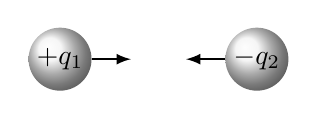
\begin{tikzpicture}[scale=1]
                \shade[ball color=gray!10!] (0,0) coordinate(q1) circle (.4) node{$+q_1$};
                \shade[ball color=gray!10!] (2.5,0) coordinate(q2) circle (.4) node{$-q_2$};
                \draw[-latex,thick] (q1)++(0.4,0)--+(0.5,0);
                \draw[-latex,thick] (q2)++(-0.4,0)--++(-0.5,0);
            \end{tikzpicture}\\[4pt]
            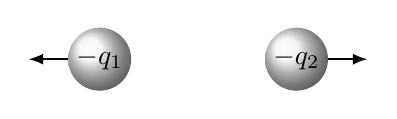
\begin{tikzpicture}[scale=1]
                \shade[ball color=gray!10!] (0,0) coordinate(q1) circle (.4) node{$-q_1$};
                \shade[ball color=gray!10!] (2.5,0) coordinate(q2) circle (.4) node{$-q_2$};
                \draw[-latex,thick] (q1)++(-0.4,0)--+(-0.5,0);
                \draw[-latex,thick] (q2)++(0.4,0)--++(0.5,0);
            \end{tikzpicture}
        \end{center}
    \end{column}
    \end{columns}
\end{frame}

\begin{frame}{Campo eléctrico} 
    El campo eléctrico es la región del espacio en el que un cuerpo o partícula cargada tiene influencia, 
    dentro de esta regíon se ejercería una fuerza sobre otros cuerpos o partículas cargadas.  
    \begin{equation*}
        E = k\dfrac{q}{r^2}
    \end{equation*}
    donde $E$ es el campo eléctrico en newtons por coulomb (\si{\newton/\coulomb}) 
    o voltios por metro (\si{\volt/\meter}), $k$ es la constante de Coulomb ($\SI{9e9}{\newton \meter\squared / \coulomb \squared}$), 
    $q$ es la carga en coulombs (\si{\coulomb}), y $r$ es la distancia entre el punto en el que se mide el campo y la carga en (\si{\meter})   
\end{frame}

\tikzset{
    carga/.style={
        circle,
        draw=azulTEC,
        line width=0.8pt,
        minimum size=6mm,
        inner sep=0pt,
        shade,
        ball color=gray!15,
        font=\scriptsize
    },
    campo/.style={
        azulTEC,
        line width=0.7pt,
        postaction={decorate},
        decoration={
            markings,
            mark=at position 0.62 with {
                \arrow{Latex[length=1.7mm,width=1.2mm]}
            }
        }
    },
    campo inverso/.style={
        azulTEC,
        line width=0.7pt,
        postaction={decorate},
        decoration={
            markings,
            mark=at position 0.38 with {
                \arrowreversed{Latex[length=1.7mm,width=1.2mm]}
            }
        }
    }
}


\begin{frame}{Líneas de campo eléctrico}

    \begin{columns}[T,onlytextwidth]

    % =========================================================
    % 1. UNA CARGA POSITIVA
    % =========================================================
    \column{0.30\textwidth}

    \centering
    \textbf{a) Una carga positiva}

    \vspace{0.4em}

    \resizebox{0.92\linewidth}{!}{%
    \begin{tikzpicture}

        \node[carga] (q) at (0,0) {$+$};

        \foreach \angulo in {0,22.5,...,337.5}{
            \draw[campo]
                (q.center)
                -- ++(\angulo:2.2);
        }

        \node[
            azulTEC,
            font=\small
        ] at (1.20,1.15) {$\vec{E}$};

    \end{tikzpicture}
    }

    \vspace{0.5em}

    {\scriptsize
    Las líneas de campo salen radialmente de una carga positiva.
    }

    % =========================================================
    % 2. DIPOLO
    % =========================================================
    \column{0.36\textwidth}

    \centering
    \textbf{b) Dos cargas iguales y opuestas}

    \vspace{0.4em}
    \resizebox{\linewidth}{!}{%
    \begin{tikzpicture}

        \node[carga] (qp) at (-1.35,0) {$+$};
        \node[carga] (qn) at ( 1.35,0) {$-$};

        % Línea central
        \draw[campo] (qp.east) -- (qn.west);

        % Líneas interiores
        \draw[campo] (qp.18)  .. controls (-0.55,0.35) and (0.55,0.35) .. (qn.162);
        \draw[campo] (qp.35)  .. controls (-0.45,0.85) and (0.45,0.85) .. (qn.145);
        \draw[campo] (qp.52)  .. controls (-0.55,1.35) and (0.55,1.35) .. (qn.128);
        \draw[campo] (qp.70)  .. controls (-0.75,1.95) and (0.75,1.95) .. (qn.110);

        \draw[campo] (qp.-18) .. controls (-0.55,-0.35) and (0.55,-0.35) .. (qn.198);
        \draw[campo] (qp.-35) .. controls (-0.45,-0.85) and (0.45,-0.85) .. (qn.215);
        \draw[campo] (qp.-52) .. controls (-0.55,-1.35) and (0.55,-1.35) .. (qn.232);
        \draw[campo] (qp.-70) .. controls (-0.75,-1.95) and (0.75,-1.95) .. (qn.250);

        % Líneas exteriores superiores (abriéndose hacia afuera)
        \draw[campo]
            (qp.95) .. controls (-2.70,1.40) and (-2.90,2.80) ..
            (0.00,3.20) ..
            controls (2.90,2.80) and (2.70,1.40) ..
            (qn.85);

        \draw[campo]
            (qp.115) .. controls (-3.05,1.20) and (-3.30,2.30) ..
            (0.00,2.75) ..
            controls (3.30,2.30) and (3.05,1.20) ..
            (qn.65);

        \draw[campo]
            (qp.135) .. controls (-3.20,0.85) and (-3.45,1.65) ..
            (0.00,2.10) ..
            controls (3.45,1.65) and (3.20,0.85) ..
            (qn.45);

        % Líneas exteriores inferiores (abriéndose hacia afuera)
        \draw[campo]
            (qp.265) .. controls (-2.70,-1.40) and (-2.90,-2.80) ..
            (0.00,-3.20) ..
            controls (2.90,-2.80) and (2.70,-1.40) ..
            (qn.275);

        \draw[campo]
            (qp.245) .. controls (-3.05,-1.20) and (-3.30,-2.30) ..
            (0.00,-2.75) ..
            controls (3.30,-2.30) and (3.05,-1.20) ..
            (qn.295);

        \draw[campo]
            (qp.225) .. controls (-3.20,-0.85) and (-3.45,-1.65) ..
            (0.00,-2.10) ..
            controls (3.45,-1.65) and (3.20,-0.85) ..
            (qn.315);

    \end{tikzpicture}
    }

    \vspace{0.5em}

    {\scriptsize
    Las líneas parten de la carga positiva y terminan en la negativa.
    }

    % =========================================================
    % 3. DOS CARGAS POSITIVAS
    % =========================================================
    \column{0.34\textwidth}

    \centering
    \textbf{c) Dos cargas positivas iguales}

    \vspace{0.4em}

    \resizebox{\linewidth}{!}{%
    \begin{tikzpicture}

        \node[carga] (q1) at (-1.35,0) {$+$};
        \node[carga] (q2) at ( 1.35,0) {$+$};

        % Horizontales exteriores
        \draw[campo inverso]
            (-3.40,0)
            -- (q1.west);

        \draw[campo]
            (q2.east)
            -- (3.40,0);

        % Carga izquierda: parte superior
        \draw[campo inverso]
            (-3.15,1.25)
            .. controls (-2.55,1.05) and (-2.25,0.70) ..
            (q1.150);

        \draw[campo inverso]
            (-2.70,2.25)
            .. controls (-2.15,1.65) and (-1.95,1.15) ..
            (q1.120);

        \draw[campo inverso]
            (-1.75,2.75)
            .. controls (-1.60,2.00) and (-1.50,1.35) ..
            (q1.95);

        % Carga izquierda: parte inferior
        \draw[campo inverso]
            (-3.15,-1.25)
            .. controls (-2.55,-1.05) and (-2.25,-0.70) ..
            (q1.210);

        \draw[campo inverso]
            (-2.70,-2.25)
            .. controls (-2.15,-1.65) and (-1.95,-1.15) ..
            (q1.240);

        \draw[campo inverso]
            (-1.75,-2.75)
            .. controls (-1.60,-2.00) and (-1.50,-1.35) ..
            (q1.265);

        % Carga derecha: parte superior
        \draw[campo]
            (q2.30)
            .. controls (2.25,0.70) and (2.55,1.05) ..
            (3.15,1.25);

        \draw[campo]
            (q2.60)
            .. controls (1.95,1.15) and (2.15,1.65) ..
            (2.70,2.25);

        \draw[campo]
            (q2.85)
            .. controls (1.50,1.35) and (1.60,2.00) ..
            (1.75,2.75);

        % Carga derecha: parte inferior
        \draw[campo]
            (q2.330)
            .. controls (2.25,-0.70) and (2.55,-1.05) ..
            (3.15,-1.25);

        \draw[campo]
            (q2.300)
            .. controls (1.95,-1.15) and (2.15,-1.65) ..
            (2.70,-2.25);

        \draw[campo]
            (q2.275)
            .. controls (1.50,-1.35) and (1.60,-2.00) ..
            (1.75,-2.75);

        % Líneas interiores que se separan
        \draw[campo]
            (q1.35)
            .. controls (-0.65,0.25) and (-0.55,1.05) ..
            (-0.35,2.75);

        \draw[campo]
            (q1.325)
            .. controls (-0.65,-0.25) and (-0.55,-1.05) ..
            (-0.35,-2.75);

        \draw[campo]
            (q2.145)
            .. controls (0.65,0.25) and (0.55,1.05) ..
            (0.35,2.75);

        \draw[campo]
            (q2.215)
            .. controls (0.65,-0.25) and (0.55,-1.05) ..
            (0.35,-2.75);

        \node[
            azulTEC,
            font=\small
        ] at (-2.20,1.10) {$\vec{E}$};

    \end{tikzpicture}
    }

    \vspace{0.5em}

    {\scriptsize
    Las líneas se separan y no cruzan el punto medio entre las cargas.
    }

    \end{columns}

\end{frame}

% \begin{frame}{Referencias}

% \bibliographystyle{ieeetr}

% \bibliography{referencias}

% \end{frame}

\end{document}